%!TEX root=../../root.tex

\section{Lezione 12}
\subsection{PDA e DPDA}
\subparagraph{Esempi} Siano $L_1$ e $L_2$ i seguenti linguaggi:
\begin{description}
	\item $L_1 = \{ w\#w^R | w \in \{0,1\}^{\star}\}$, ossia l'insieme delle parole palindrome con un $\#$ al centro. \\
	\begin{figure}[H]
		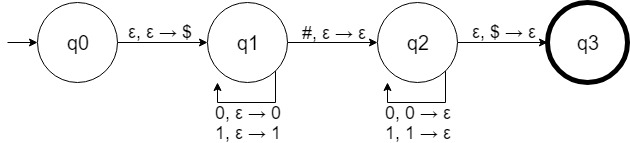
\includegraphics[scale=0.5]{pda1}
	\end{figure}
	\item $L_2 = \{ ww^R | w \in \{0,1\}^{\star}\}$, ossia l'insieme delle parole palindrome di lunghezza pari. \\
	\begin{figure}[H]
		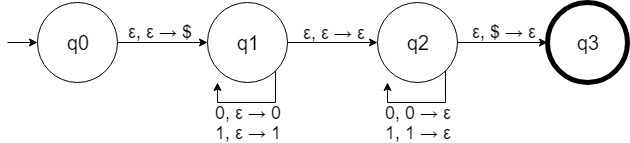
\includegraphics[scale=0.5]{pda2}
	\end{figure}
\end{description}
Nel linguaggio $L_1$ sappiamo quando abbiamo finito di leggere $w$ appena leggiamo $\#$ in input. A questo punto abbiamo $w$ impilata nella pila dell'automa e possiamo controllare che il resto dell'input sia esattamente $w$ al contrario.\\
Nel linguaggio $L_2$ invece non sappiamo con certezza quale sia il carattere che determina la fine della parola $w$ per tale motivo dobbiamo ricorrere al non determinismo. Infatti l'automa ha sempre la possibilit\`a di fare o non fare la $\varepsilon$ mossa. Quindi in $q_1$ ho sempre due possibilit\`a: continuare ad impilare oppure iniziare a togliere dalla pila. \\
Nei PDA il modello non deterministico è molto più potente dell'equivalente deterministico, infatti abbiamo che: 
\[ 
	L(DPDA) \subsetneq L(PDA)
\]
Questo è l'unico modello in cui questo è vero.\\
\textit{Dimostrazione:}
Dato un automa a pila deterministico $A = (Q,\Sigma,\Gamma,\delta,q_{0},F)$ la cui funzione di transizione è definita come segue:
\[
	\delta: Q\times \Sigma_{\varepsilon}\times\Gamma_{\varepsilon} \to {\cal P} (Q\times \Gamma_{\varepsilon})
\]
Affinch\'e A sia deterministico deve valere che:
\begin{enumerate}
	\item $|\delta(q,a,A)| \leq 1 \quad \forall  a \in \Sigma_{\varepsilon}, \forall A \in \Gamma_{\varepsilon}$
	\item $|\delta(q,\varepsilon,A)| = 1 \Rightarrow  \delta(q,a,A) = \emptyset \quad \forall  a \in \Sigma, \ \forall A \in \Gamma_{\varepsilon}$, ossia se da $q$ leggendo in input $\varepsilon$ e sulla cima della pila $A$ l'automa effettua una transizione allora da $q$ leggendo $A$ dalla pila e qualsiasi altro carattere in input l'automa non deve effettuare transizioni.
	\item $|\delta(q,a,\varepsilon)| = 1 \Rightarrow  \delta(q,a,A) = \emptyset \quad \forall  a \in \Sigma_{\varepsilon}, \ \forall A \in \Gamma$, ossia se da $q$ leggendo $a$ in input e la parola vuota dalla cima della pila l'automa effettua una transizione allora se in cima alla pila c'è un carattere diverso da $\varepsilon$ allora l'automa non deve effettuare transizioni.
\end{enumerate}

\subsection{Equivalenza tra linguaggi generati da PDA e CFL}
Si vuole dimostrare che $L(PDA) \textbf{=} L(CFG) = CFL$. 
\begin{enumerate}
	\item $L(PDA) \subseteq CFL$, non sar\`a trattata in questo documento.
	\item $CFL \subseteq L(PDA)$, utile dimostrazione poich\'e usa la stessa tecnica per costruire i parser di linguaggi di programmazione. \\
		Quindi vogliamo dimostrare che: $L \in L(CFL) \Rightarrow L \in L(PDA)$
\end{enumerate} 
\textit{Dimostrazione:}
Se $L \in L(CFL)$ allora $\exists \ G = \ (V,\Sigma,R,S) \ | \ L(G) \ = \ L $. Il seguente $PDA$ è costruito in modo da accettare il linguaggio denotato dalla grammatica G, quindi accetta il linguaggio $L$.
\begin{figure}[H]
	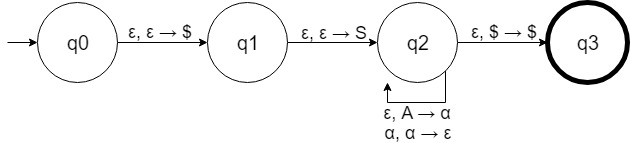
\includegraphics[scale=0.5]{pda3}
\end{figure}
\begin{description}
	\item \textit{Esempio:} Data la grammatica $G = (\{S,A\}, \{a, b\}, \{S \to aSA | \varepsilon, A \to bA | b\}, S )$ costruiamo il $PDA$ che riconosce il linguaggio descritto da $G$. \\
% Immagine		
\end{description}

\newpage 

\subsection{Modello di Turing}
Una macchina di Turing è caratterizzata da:
\begin{itemize}
	\item Un nastro di input con lunghezza infinita a destra, formato da celle che possono memorizzare un carattere l'una. Tra i caratteri vi è un carattere speciale utilizzato per indicare la cella vuota, detto blank, indicato con "B".
	\item Una testina per la lettura e la scrittura di caratteri sul nastro, la quale si pu\`o muovere sia a destra che a sinistra o restare ferma.
	\item Un insieme finito di stati in cui pu\`o transitare, fra cui uno stato iniziale $q_0$, lo stato di accettazione $q_a$ e lo stato di rifiuto $q_r$
\end{itemize}
\paragraph{Modello Formale} Sia M una macchina di Turing, essa è definita come la seguente 7-tupla
\[
	M = (Q,\Sigma,\Gamma,\delta,q_0,q_a,q_r) 
\]
Dove:
\begin{itemize}
	\item Q: insieme finito di stati di M
	\item $\Sigma \subseteq \Gamma$: alfabeto finito di input 
	\item $\Gamma$: alfabeto finito di nastro
	\item $\delta: Q\times\Gamma \to Q \times \Gamma \times\{L,R\}$: funzione di transizione
\end{itemize}
Anche in questo modello possiamo definire il concetto di \textit{configurazione}. Una configurazione deve mantenere le seguenti informazioni:
\begin{itemize}
	\item stato attuale 
	\item contenuto del nastro $\alpha \in \Gamma^{\star}$
	\item posizione della testina sul nastro
\end{itemize}
Sia $c$ una configurazione generica 
$$
c = \alpha p a \beta \text{ con }\alpha, \beta \in \Gamma^{\star} \ a \in \Gamma,  p \in Q
$$
essa ci fornisce le seguenti informazioni:
\begin{itemize}
	\item la macchina si trova sullo stato $p$
	\item il contenuto del nastro è $\alpha a \beta$
	\item la testina è posizionata sulla cella di $a$ (il primo carattere dopo lo stato)
\end{itemize}
Per descrivere un passo di calcolo abbiamo bisogno di definire una relazione ($\Rightarrow_M$) tra due configurazioni. Sia $c' = \alpha b q \beta$ un'altra configurazione dove $\alpha$ e $\beta$ sono le stesse di $c$, mentre $b \in \Gamma$ e $q \in Q$ potrebbero essere differenti. Le due configurazioni sono in relazione se da $c$ con un passo di calcolo si può raggiungere $c'$:
\[
	\text{Se }\delta(p,a) = (q, b, R) \text{ allora scriviamo } \alpha p a \beta \Rightarrow_M \alpha b q \beta \text{ ossia }  c \Rightarrow_M c' 
\]
Quindi dallo stato $p$ leggendo $a$ sul nastro viene scritto $b$ al posto di $a$ e viene fatto un passo a destra spostando la testina sul primo carattere di $\beta$ (non necessario esplicitarlo) e l'automa transita nello stato $q$.

Come al solito definiamo anche la chiusura riflessiva e transitiva di $\Rightarrow_M$ che ci aiuta nella definizione del linguaggio accettato dalla macchina $M$.
\[
	L(M) = \{ x \ | \ x \in \Sigma^{\star} \land q_0 x \Rightarrow_M^{\star} \alpha q_a\beta \text{ con } \alpha, \beta \in \Gamma^{\star}\}
\]
\subsection{Correlazione tra problemi di decisione e di ricerca}
Un \textit{problema di decisione} è un problema che risponde in modo dicotomico ad una certa domanda. Ad esempio dato un grafo stabilire se esiste un cammino aciclico. Invece un \textit{problema di ricerca} è un problema che trova un' istanza che soddisfi una certa domanda. Ad esempio dato un grafo esibire un cammino aciclico.

Vediamo ora il problema della ricerca di un assegnamento per una formula booleana che la renda soddisfatta. Partiamo dal problema di decisione correlato, ossia stabilire se esiste un assegnamento che renda soddisfatta la formula.
\\

\textbf{ALGSAT:}
\begin{description}
	\item \textit{Input:} $\varphi$, formula booleana
	\item \textit{Output:} "s\`i" se $\varphi$ è soddisfacibile, "no" altrimenti.
	\item \textit{Algoritmo:} ricerca esaustiva di un assegnamento. Nel caso peggiore se $\varphi$ è formata da $k$ variabili allora verranno generate $2^k$ stringhe binarie da testare.
\end{description}
Ora definiamo un algoritmo di ricerca che utilizza \textit{ALGSAT}:
\\

\textbf{ALGRICSAT:}
\begin{description}
	\item \textit{Input:} $\varphi$, formula booleana
	\item \textit{Output:} un assegnamento che soddisfa $\varphi$ se esiste, altrimenti "no".
	\item \textit{Algoritmo:}
		\begin{enumerate}
			\item esegui \textit{ALGSAT}. Se risponde "no" allora termina e rispondi "no", altrimenti continua.
			\item Si assegna 0 alla prima variabile e si esegue \textit{ALGSAT} sulla formula ottenuta $\varphi_0$. Se $\varphi_0$ non e' soddisfacibile si pone la prima variabile a 1.
			\item In entrambi i casi si prosegue nello stesso modo per la successive variabili.
			 
		\end{enumerate}
\end{description}
